% This is a Basic Assignment Paper but with like Code and stuff allowed in it, there is also url, hyperlinks from contents included. 

\documentclass[11pt]{article}

% Preamble

\usepackage[margin=1in]{geometry}
\usepackage{amsfonts, amsmath, amssymb}
\usepackage{fancyhdr, float, graphicx}
\usepackage[utf8]{inputenc} % Required for inputting international characters
\usepackage[T1]{fontenc} % Output font encoding for international characters
\usepackage{fouriernc} % Use the New Century Schoolbook font
\usepackage[nottoc, notlot, notlof]{tocbibind}
\usepackage{listings}
\usepackage{xcolor}
\usepackage{blindtext}
\usepackage{hyperref}


\definecolor{codegreen}{rgb}{0,0.6,0}
\definecolor{codegray}{rgb}{0.5,0.5,0.5}
\definecolor{codepurple}{rgb}{0.58,0,0.82}
\definecolor{backcolour}{rgb}{0.95,0.95,0.92}

\lstdefinestyle{mystyle}{
    backgroundcolor=\color{backcolour},   
    commentstyle=\color{codegreen},
    keywordstyle=\color{magenta},
    numberstyle=\tiny\color{codegray},
    stringstyle=\color{codepurple},
    basicstyle=\ttfamily\footnotesize,
    breakatwhitespace=false,         
    breaklines=true,                 
    captionpos=b,                    
    keepspaces=true,                 
    numbers=left,                    
    numbersep=5pt,                  
    showspaces=false,                
    showstringspaces=false,
    showtabs=false,                  
    tabsize=2
}

\lstset{style=mystyle}

% Header and Footer
\pagestyle{fancy}
\fancyhead{}
\fancyfoot{}
\fancyhead[L]{\textit{\Large{Python Programming Assignment 11}}}
%\fancyhead[R]{\textit{something}}
\fancyfoot[C]{\thepage}
\renewcommand{\footrulewidth}{1pt}

\usepackage[breakable]{tcolorbox}
\usepackage{parskip} % Stop auto-indenting (to mimic markdown behaviour)


% Basic figure setup, for now with no caption control since it's done
% automatically by Pandoc (which extracts ![](path) syntax from Markdown).
\usepackage{graphicx}
% Maintain compatibility with old templates. Remove in nbconvert 6.0
\let\Oldincludegraphics\includegraphics
% Ensure that by default, figures have no caption (until we provide a
% proper Figure object with a Caption API and a way to capture that
% in the conversion process - todo).
\usepackage{caption}
\DeclareCaptionFormat{nocaption}{}
\captionsetup{format=nocaption,aboveskip=0pt,belowskip=0pt}

\usepackage{float}
\floatplacement{figure}{H} % forces figures to be placed at the correct location
\usepackage{xcolor} % Allow colors to be defined
\usepackage{enumerate} % Needed for markdown enumerations to work
\usepackage{geometry} % Used to adjust the document margins
\usepackage{amsmath} % Equations
\usepackage{amssymb} % Equations
\usepackage{textcomp} % defines textquotesingle
% Hack from http://tex.stackexchange.com/a/47451/13684:
\AtBeginDocument{%
	\def\PYZsq{\textquotesingle}% Upright quotes in Pygmentized code
}
\usepackage{upquote} % Upright quotes for verbatim code
\usepackage{eurosym} % defines \euro

\usepackage{iftex}
% \ifPDFTeX
% 	\usepackage[T1]{fontenc}
% 	\IfFileExists{alphabeta.sty}{
% 		  \usepackage{alphabeta}
% 	  }{
% 		  \usepackage[mathletters]{ucs}
% 		  \usepackage[utf8x]{inputenc}
% 	  }
% \else
% 	\usepackage{fontspec}
% 	\usepackage{unicode-math}
% \fi

\usepackage{fancyvrb} % verbatim replacement that allows latex
\usepackage{grffile} % extends the file name processing of package graphics
					 % to support a larger range
\makeatletter % fix for old versions of grffile with XeLaTeX
\@ifpackagelater{grffile}{2019/11/01}
{
  % Do nothing on new versions
}
{
  \def\Gread@@xetex#1{%
	\IfFileExists{"\Gin@base".bb}%
	{\Gread@eps{\Gin@base.bb}}%
	{\Gread@@xetex@aux#1}%
  }
}
\makeatother
\usepackage[Export]{adjustbox} % Used to constrain images to a maximum size
\adjustboxset{max size={0.9\linewidth}{0.9\paperheight}}

% The hyperref package gives us a pdf with properly built
% internal navigation ('pdf bookmarks' for the table of contents,
% internal cross-reference links, web links for URLs, etc.)
\usepackage{hyperref}
% The default LaTeX title has an obnoxious amount of whitespace. By default,
% titling removes some of it. It also provides customization options.
\usepackage{titling}
\usepackage{longtable} % longtable support required by pandoc >1.10
\usepackage{booktabs}  % table support for pandoc > 1.12.2
\usepackage{array}     % table support for pandoc >= 2.11.3
\usepackage{calc}      % table minipage width calculation for pandoc >= 2.11.1
\usepackage[inline]{enumitem} % IRkernel/repr support (it uses the enumerate* environment)
\usepackage[normalem]{ulem} % ulem is needed to support strikethroughs (\sout)
							% normalem makes italics be italics, not underlines
\usepackage{mathrsfs}



% Colors for the hyperref package
\definecolor{urlcolor}{rgb}{0,.145,.698}
\definecolor{linkcolor}{rgb}{.71,0.21,0.01}
\definecolor{citecolor}{rgb}{.12,.54,.11}

% ANSI colors
\definecolor{ansi-black}{HTML}{3E424D}
\definecolor{ansi-black-intense}{HTML}{282C36}
\definecolor{ansi-red}{HTML}{E75C58}
\definecolor{ansi-red-intense}{HTML}{B22B31}
\definecolor{ansi-green}{HTML}{00A250}
\definecolor{ansi-green-intense}{HTML}{007427}
\definecolor{ansi-yellow}{HTML}{DDB62B}
\definecolor{ansi-yellow-intense}{HTML}{B27D12}
\definecolor{ansi-blue}{HTML}{208FFB}
\definecolor{ansi-blue-intense}{HTML}{0065CA}
\definecolor{ansi-magenta}{HTML}{D160C4}
\definecolor{ansi-magenta-intense}{HTML}{A03196}
\definecolor{ansi-cyan}{HTML}{60C6C8}
\definecolor{ansi-cyan-intense}{HTML}{258F8F}
\definecolor{ansi-white}{HTML}{C5C1B4}
\definecolor{ansi-white-intense}{HTML}{A1A6B2}
\definecolor{ansi-default-inverse-fg}{HTML}{FFFFFF}
\definecolor{ansi-default-inverse-bg}{HTML}{000000}

% common color for the border for error outputs.
\definecolor{outerrorbackground}{HTML}{FFDFDF}

% commands and environments needed by pandoc snippets
% extracted from the output of `pandoc -s`
\providecommand{\tightlist}{%
  \setlength{\itemsep}{0pt}\setlength{\parskip}{0pt}}
\DefineVerbatimEnvironment{Highlighting}{Verbatim}{commandchars=\\\{\}}
% Add ',fontsize=\small' for more characters per line
\newenvironment{Shaded}{}{}
\newcommand{\KeywordTok}[1]{\textcolor[rgb]{0.00,0.44,0.13}{\textbf{{#1}}}}
\newcommand{\DataTypeTok}[1]{\textcolor[rgb]{0.56,0.13,0.00}{{#1}}}
\newcommand{\DecValTok}[1]{\textcolor[rgb]{0.25,0.63,0.44}{{#1}}}
\newcommand{\BaseNTok}[1]{\textcolor[rgb]{0.25,0.63,0.44}{{#1}}}
\newcommand{\FloatTok}[1]{\textcolor[rgb]{0.25,0.63,0.44}{{#1}}}
\newcommand{\CharTok}[1]{\textcolor[rgb]{0.25,0.44,0.63}{{#1}}}
\newcommand{\StringTok}[1]{\textcolor[rgb]{0.25,0.44,0.63}{{#1}}}
\newcommand{\CommentTok}[1]{\textcolor[rgb]{0.38,0.63,0.69}{\textit{{#1}}}}
\newcommand{\OtherTok}[1]{\textcolor[rgb]{0.00,0.44,0.13}{{#1}}}
\newcommand{\AlertTok}[1]{\textcolor[rgb]{1.00,0.00,0.00}{\textbf{{#1}}}}
\newcommand{\FunctionTok}[1]{\textcolor[rgb]{0.02,0.16,0.49}{{#1}}}
\newcommand{\RegionMarkerTok}[1]{{#1}}
\newcommand{\ErrorTok}[1]{\textcolor[rgb]{1.00,0.00,0.00}{\textbf{{#1}}}}
\newcommand{\NormalTok}[1]{{#1}}

% Additional commands for more recent versions of Pandoc
\newcommand{\ConstantTok}[1]{\textcolor[rgb]{0.53,0.00,0.00}{{#1}}}
\newcommand{\SpecialCharTok}[1]{\textcolor[rgb]{0.25,0.44,0.63}{{#1}}}
\newcommand{\VerbatimStringTok}[1]{\textcolor[rgb]{0.25,0.44,0.63}{{#1}}}
\newcommand{\SpecialStringTok}[1]{\textcolor[rgb]{0.73,0.40,0.53}{{#1}}}
\newcommand{\ImportTok}[1]{{#1}}
\newcommand{\DocumentationTok}[1]{\textcolor[rgb]{0.73,0.13,0.13}{\textit{{#1}}}}
\newcommand{\AnnotationTok}[1]{\textcolor[rgb]{0.38,0.63,0.69}{\textbf{\textit{{#1}}}}}
\newcommand{\CommentVarTok}[1]{\textcolor[rgb]{0.38,0.63,0.69}{\textbf{\textit{{#1}}}}}
\newcommand{\VariableTok}[1]{\textcolor[rgb]{0.10,0.09,0.49}{{#1}}}
\newcommand{\ControlFlowTok}[1]{\textcolor[rgb]{0.00,0.44,0.13}{\textbf{{#1}}}}
\newcommand{\OperatorTok}[1]{\textcolor[rgb]{0.40,0.40,0.40}{{#1}}}
\newcommand{\BuiltInTok}[1]{{#1}}
\newcommand{\ExtensionTok}[1]{{#1}}
\newcommand{\PreprocessorTok}[1]{\textcolor[rgb]{0.74,0.48,0.00}{{#1}}}
\newcommand{\AttributeTok}[1]{\textcolor[rgb]{0.49,0.56,0.16}{{#1}}}
\newcommand{\InformationTok}[1]{\textcolor[rgb]{0.38,0.63,0.69}{\textbf{\textit{{#1}}}}}
\newcommand{\WarningTok}[1]{\textcolor[rgb]{0.38,0.63,0.69}{\textbf{\textit{{#1}}}}}


% Define a nice break command that doesn't care if a line doesn't already
% exist.
\def\br{\hspace*{\fill} \\* }
% Math Jax compatibility definitions
\def\gt{>}
\def\lt{<}
\let\Oldtex\TeX
\let\Oldlatex\LaTeX
\renewcommand{\TeX}{\textrm{\Oldtex}}
\renewcommand{\LaTeX}{\textrm{\Oldlatex}}
% Document parameters
% Document title
\title{Assignment\_1}





% Pygments definitions
\makeatletter
\def\PY@reset{\let\PY@it=\relax \let\PY@bf=\relax%
\let\PY@ul=\relax \let\PY@tc=\relax%
\let\PY@bc=\relax \let\PY@ff=\relax}
\def\PY@tok#1{\csname PY@tok@#1\endcsname}
\def\PY@toks#1+{\ifx\relax#1\empty\else%
\PY@tok{#1}\expandafter\PY@toks\fi}
\def\PY@do#1{\PY@bc{\PY@tc{\PY@ul{%
\PY@it{\PY@bf{\PY@ff{#1}}}}}}}
\def\PY#1#2{\PY@reset\PY@toks#1+\relax+\PY@do{#2}}

\@namedef{PY@tok@w}{\def\PY@tc##1{\textcolor[rgb]{0.73,0.73,0.73}{##1}}}
\@namedef{PY@tok@c}{\let\PY@it=\textit\def\PY@tc##1{\textcolor[rgb]{0.24,0.48,0.48}{##1}}}
\@namedef{PY@tok@cp}{\def\PY@tc##1{\textcolor[rgb]{0.61,0.40,0.00}{##1}}}
\@namedef{PY@tok@k}{\let\PY@bf=\textbf\def\PY@tc##1{\textcolor[rgb]{0.00,0.50,0.00}{##1}}}
\@namedef{PY@tok@kp}{\def\PY@tc##1{\textcolor[rgb]{0.00,0.50,0.00}{##1}}}
\@namedef{PY@tok@kt}{\def\PY@tc##1{\textcolor[rgb]{0.69,0.00,0.25}{##1}}}
\@namedef{PY@tok@o}{\def\PY@tc##1{\textcolor[rgb]{0.40,0.40,0.40}{##1}}}
\@namedef{PY@tok@ow}{\let\PY@bf=\textbf\def\PY@tc##1{\textcolor[rgb]{0.67,0.13,1.00}{##1}}}
\@namedef{PY@tok@nb}{\def\PY@tc##1{\textcolor[rgb]{0.00,0.50,0.00}{##1}}}
\@namedef{PY@tok@nf}{\def\PY@tc##1{\textcolor[rgb]{0.00,0.00,1.00}{##1}}}
\@namedef{PY@tok@nc}{\let\PY@bf=\textbf\def\PY@tc##1{\textcolor[rgb]{0.00,0.00,1.00}{##1}}}
\@namedef{PY@tok@nn}{\let\PY@bf=\textbf\def\PY@tc##1{\textcolor[rgb]{0.00,0.00,1.00}{##1}}}
\@namedef{PY@tok@ne}{\let\PY@bf=\textbf\def\PY@tc##1{\textcolor[rgb]{0.80,0.25,0.22}{##1}}}
\@namedef{PY@tok@nv}{\def\PY@tc##1{\textcolor[rgb]{0.10,0.09,0.49}{##1}}}
\@namedef{PY@tok@no}{\def\PY@tc##1{\textcolor[rgb]{0.53,0.00,0.00}{##1}}}
\@namedef{PY@tok@nl}{\def\PY@tc##1{\textcolor[rgb]{0.46,0.46,0.00}{##1}}}
\@namedef{PY@tok@ni}{\let\PY@bf=\textbf\def\PY@tc##1{\textcolor[rgb]{0.44,0.44,0.44}{##1}}}
\@namedef{PY@tok@na}{\def\PY@tc##1{\textcolor[rgb]{0.41,0.47,0.13}{##1}}}
\@namedef{PY@tok@nt}{\let\PY@bf=\textbf\def\PY@tc##1{\textcolor[rgb]{0.00,0.50,0.00}{##1}}}
\@namedef{PY@tok@nd}{\def\PY@tc##1{\textcolor[rgb]{0.67,0.13,1.00}{##1}}}
\@namedef{PY@tok@s}{\def\PY@tc##1{\textcolor[rgb]{0.73,0.13,0.13}{##1}}}
\@namedef{PY@tok@sd}{\let\PY@it=\textit\def\PY@tc##1{\textcolor[rgb]{0.73,0.13,0.13}{##1}}}
\@namedef{PY@tok@si}{\let\PY@bf=\textbf\def\PY@tc##1{\textcolor[rgb]{0.64,0.35,0.47}{##1}}}
\@namedef{PY@tok@se}{\let\PY@bf=\textbf\def\PY@tc##1{\textcolor[rgb]{0.67,0.36,0.12}{##1}}}
\@namedef{PY@tok@sr}{\def\PY@tc##1{\textcolor[rgb]{0.64,0.35,0.47}{##1}}}
\@namedef{PY@tok@ss}{\def\PY@tc##1{\textcolor[rgb]{0.10,0.09,0.49}{##1}}}
\@namedef{PY@tok@sx}{\def\PY@tc##1{\textcolor[rgb]{0.00,0.50,0.00}{##1}}}
\@namedef{PY@tok@m}{\def\PY@tc##1{\textcolor[rgb]{0.40,0.40,0.40}{##1}}}
\@namedef{PY@tok@gh}{\let\PY@bf=\textbf\def\PY@tc##1{\textcolor[rgb]{0.00,0.00,0.50}{##1}}}
\@namedef{PY@tok@gu}{\let\PY@bf=\textbf\def\PY@tc##1{\textcolor[rgb]{0.50,0.00,0.50}{##1}}}
\@namedef{PY@tok@gd}{\def\PY@tc##1{\textcolor[rgb]{0.63,0.00,0.00}{##1}}}
\@namedef{PY@tok@gi}{\def\PY@tc##1{\textcolor[rgb]{0.00,0.52,0.00}{##1}}}
\@namedef{PY@tok@gr}{\def\PY@tc##1{\textcolor[rgb]{0.89,0.00,0.00}{##1}}}
\@namedef{PY@tok@ge}{\let\PY@it=\textit}
\@namedef{PY@tok@gs}{\let\PY@bf=\textbf}
\@namedef{PY@tok@gp}{\let\PY@bf=\textbf\def\PY@tc##1{\textcolor[rgb]{0.00,0.00,0.50}{##1}}}
\@namedef{PY@tok@go}{\def\PY@tc##1{\textcolor[rgb]{0.44,0.44,0.44}{##1}}}
\@namedef{PY@tok@gt}{\def\PY@tc##1{\textcolor[rgb]{0.00,0.27,0.87}{##1}}}
\@namedef{PY@tok@err}{\def\PY@bc##1{{\setlength{\fboxsep}{\string -\fboxrule}\fcolorbox[rgb]{1.00,0.00,0.00}{1,1,1}{\strut ##1}}}}
\@namedef{PY@tok@kc}{\let\PY@bf=\textbf\def\PY@tc##1{\textcolor[rgb]{0.00,0.50,0.00}{##1}}}
\@namedef{PY@tok@kd}{\let\PY@bf=\textbf\def\PY@tc##1{\textcolor[rgb]{0.00,0.50,0.00}{##1}}}
\@namedef{PY@tok@kn}{\let\PY@bf=\textbf\def\PY@tc##1{\textcolor[rgb]{0.00,0.50,0.00}{##1}}}
\@namedef{PY@tok@kr}{\let\PY@bf=\textbf\def\PY@tc##1{\textcolor[rgb]{0.00,0.50,0.00}{##1}}}
\@namedef{PY@tok@bp}{\def\PY@tc##1{\textcolor[rgb]{0.00,0.50,0.00}{##1}}}
\@namedef{PY@tok@fm}{\def\PY@tc##1{\textcolor[rgb]{0.00,0.00,1.00}{##1}}}
\@namedef{PY@tok@vc}{\def\PY@tc##1{\textcolor[rgb]{0.10,0.09,0.49}{##1}}}
\@namedef{PY@tok@vg}{\def\PY@tc##1{\textcolor[rgb]{0.10,0.09,0.49}{##1}}}
\@namedef{PY@tok@vi}{\def\PY@tc##1{\textcolor[rgb]{0.10,0.09,0.49}{##1}}}
\@namedef{PY@tok@vm}{\def\PY@tc##1{\textcolor[rgb]{0.10,0.09,0.49}{##1}}}
\@namedef{PY@tok@sa}{\def\PY@tc##1{\textcolor[rgb]{0.73,0.13,0.13}{##1}}}
\@namedef{PY@tok@sb}{\def\PY@tc##1{\textcolor[rgb]{0.73,0.13,0.13}{##1}}}
\@namedef{PY@tok@sc}{\def\PY@tc##1{\textcolor[rgb]{0.73,0.13,0.13}{##1}}}
\@namedef{PY@tok@dl}{\def\PY@tc##1{\textcolor[rgb]{0.73,0.13,0.13}{##1}}}
\@namedef{PY@tok@s2}{\def\PY@tc##1{\textcolor[rgb]{0.73,0.13,0.13}{##1}}}
\@namedef{PY@tok@sh}{\def\PY@tc##1{\textcolor[rgb]{0.73,0.13,0.13}{##1}}}
\@namedef{PY@tok@s1}{\def\PY@tc##1{\textcolor[rgb]{0.73,0.13,0.13}{##1}}}
\@namedef{PY@tok@mb}{\def\PY@tc##1{\textcolor[rgb]{0.40,0.40,0.40}{##1}}}
\@namedef{PY@tok@mf}{\def\PY@tc##1{\textcolor[rgb]{0.40,0.40,0.40}{##1}}}
\@namedef{PY@tok@mh}{\def\PY@tc##1{\textcolor[rgb]{0.40,0.40,0.40}{##1}}}
\@namedef{PY@tok@mi}{\def\PY@tc##1{\textcolor[rgb]{0.40,0.40,0.40}{##1}}}
\@namedef{PY@tok@il}{\def\PY@tc##1{\textcolor[rgb]{0.40,0.40,0.40}{##1}}}
\@namedef{PY@tok@mo}{\def\PY@tc##1{\textcolor[rgb]{0.40,0.40,0.40}{##1}}}
\@namedef{PY@tok@ch}{\let\PY@it=\textit\def\PY@tc##1{\textcolor[rgb]{0.24,0.48,0.48}{##1}}}
\@namedef{PY@tok@cm}{\let\PY@it=\textit\def\PY@tc##1{\textcolor[rgb]{0.24,0.48,0.48}{##1}}}
\@namedef{PY@tok@cpf}{\let\PY@it=\textit\def\PY@tc##1{\textcolor[rgb]{0.24,0.48,0.48}{##1}}}
\@namedef{PY@tok@c1}{\let\PY@it=\textit\def\PY@tc##1{\textcolor[rgb]{0.24,0.48,0.48}{##1}}}
\@namedef{PY@tok@cs}{\let\PY@it=\textit\def\PY@tc##1{\textcolor[rgb]{0.24,0.48,0.48}{##1}}}

\def\PYZbs{\char`\\}
\def\PYZus{\char`\_}
\def\PYZob{\char`\{}
\def\PYZcb{\char`\}}
\def\PYZca{\char`\^}
\def\PYZam{\char`\&}
\def\PYZlt{\char`\<}
\def\PYZgt{\char`\>}
\def\PYZsh{\char`\#}
\def\PYZpc{\char`\%}
\def\PYZdl{\char`\$}
\def\PYZhy{\char`\-}
\def\PYZsq{\char`\'}
\def\PYZdq{\char`\"}
\def\PYZti{\char`\~}
% for compatibility with earlier versions
\def\PYZat{@}
\def\PYZlb{[}
\def\PYZrb{]}
\makeatother


% For linebreaks inside Verbatim environment from package fancyvrb.
\makeatletter
	\newbox\Wrappedcontinuationbox
	\newbox\Wrappedvisiblespacebox
	\newcommand*\Wrappedvisiblespace {\textcolor{red}{\textvisiblespace}}
	\newcommand*\Wrappedcontinuationsymbol {\textcolor{red}{\llap{\tiny$\m@th\hookrightarrow$}}}
	\newcommand*\Wrappedcontinuationindent {3ex }
	\newcommand*\Wrappedafterbreak {\kern\Wrappedcontinuationindent\copy\Wrappedcontinuationbox}
	% Take advantage of the already applied Pygments mark-up to insert
	% potential linebreaks for TeX processing.
	%        {, <, #, %, $, ' and ": go to next line.
	%        _, }, ^, &, >, - and ~: stay at end of broken line.
	% Use of \textquotesingle for straight quote.
	\newcommand*\Wrappedbreaksatspecials {%
		\def\PYGZus{\discretionary{\char`\_}{\Wrappedafterbreak}{\char`\_}}%
		\def\PYGZob{\discretionary{}{\Wrappedafterbreak\char`\{}{\char`\{}}%
		\def\PYGZcb{\discretionary{\char`\}}{\Wrappedafterbreak}{\char`\}}}%
		\def\PYGZca{\discretionary{\char`\^}{\Wrappedafterbreak}{\char`\^}}%
		\def\PYGZam{\discretionary{\char`\&}{\Wrappedafterbreak}{\char`\&}}%
		\def\PYGZlt{\discretionary{}{\Wrappedafterbreak\char`\<}{\char`\<}}%
		\def\PYGZgt{\discretionary{\char`\>}{\Wrappedafterbreak}{\char`\>}}%
		\def\PYGZsh{\discretionary{}{\Wrappedafterbreak\char`\#}{\char`\#}}%
		\def\PYGZpc{\discretionary{}{\Wrappedafterbreak\char`\%}{\char`\%}}%
		\def\PYGZdl{\discretionary{}{\Wrappedafterbreak\char`\$}{\char`\$}}%
		\def\PYGZhy{\discretionary{\char`\-}{\Wrappedafterbreak}{\char`\-}}%
		\def\PYGZsq{\discretionary{}{\Wrappedafterbreak\textquotesingle}{\textquotesingle}}%
		\def\PYGZdq{\discretionary{}{\Wrappedafterbreak\char`\"}{\char`\"}}%
		\def\PYGZti{\discretionary{\char`\~}{\Wrappedafterbreak}{\char`\~}}%
	}
	% Some characters . , ; ? ! / are not pygmentized.
	% This macro makes them "active" and they will insert potential linebreaks
	\newcommand*\Wrappedbreaksatpunct {%
		\lccode`\~`\.\lowercase{\def~}{\discretionary{\hbox{\char`\.}}{\Wrappedafterbreak}{\hbox{\char`\.}}}%
		\lccode`\~`\,\lowercase{\def~}{\discretionary{\hbox{\char`\,}}{\Wrappedafterbreak}{\hbox{\char`\,}}}%
		\lccode`\~`\;\lowercase{\def~}{\discretionary{\hbox{\char`\;}}{\Wrappedafterbreak}{\hbox{\char`\;}}}%
		\lccode`\~`\:\lowercase{\def~}{\discretionary{\hbox{\char`\:}}{\Wrappedafterbreak}{\hbox{\char`\:}}}%
		\lccode`\~`\?\lowercase{\def~}{\discretionary{\hbox{\char`\?}}{\Wrappedafterbreak}{\hbox{\char`\?}}}%
		\lccode`\~`\!\lowercase{\def~}{\discretionary{\hbox{\char`\!}}{\Wrappedafterbreak}{\hbox{\char`\!}}}%
		\lccode`\~`\/\lowercase{\def~}{\discretionary{\hbox{\char`\/}}{\Wrappedafterbreak}{\hbox{\char`\/}}}%
		\catcode`\.\active
		\catcode`\,\active
		\catcode`\;\active
		\catcode`\:\active
		\catcode`\?\active
		\catcode`\!\active
		\catcode`\/\active
		\lccode`\~`\~
	}
\makeatother

\let\OriginalVerbatim=\Verbatim
\makeatletter
\renewcommand{\Verbatim}[1][1]{%
	%\parskip\z@skip
	\sbox\Wrappedcontinuationbox {\Wrappedcontinuationsymbol}%
	\sbox\Wrappedvisiblespacebox {\FV@SetupFont\Wrappedvisiblespace}%
	\def\FancyVerbFormatLine ##1{\hsize\linewidth
		\vtop{\raggedright\hyphenpenalty\z@\exhyphenpenalty\z@
			\doublehyphendemerits\z@\finalhyphendemerits\z@
			\strut ##1\strut}%
	}%
	% If the linebreak is at a space, the latter will be displayed as visible
	% space at end of first line, and a continuation symbol starts next line.
	% Stretch/shrink are however usually zero for typewriter font.
	\def\FV@Space {%
		\nobreak\hskip\z@ plus\fontdimen3\font minus\fontdimen4\font
		\discretionary{\copy\Wrappedvisiblespacebox}{\Wrappedafterbreak}
		{\kern\fontdimen2\font}%
	}%

	% Allow breaks at special characters using \PYG... macros.
	\Wrappedbreaksatspecials
	% Breaks at punctuation characters . , ; ? ! and / need catcode=\active
	\OriginalVerbatim[#1,codes*=\Wrappedbreaksatpunct]%
}
\makeatother

% Exact colors from NB
\definecolor{incolor}{HTML}{303F9F}
\definecolor{outcolor}{HTML}{D84315}
\definecolor{cellborder}{HTML}{CFCFCF}
\definecolor{cellbackground}{HTML}{F7F7F7}

% prompt
\makeatletter
\newcommand{\boxspacing}{\kern\kvtcb@left@rule\kern\kvtcb@boxsep}
\makeatother
\newcommand{\prompt}[4]{
	{\ttfamily\llap{{\color{#2}[#3]:\hspace{3pt}#4}}\vspace{-\baselineskip}}
}



% Prevent overflowing lines due to hard-to-break entities
\sloppy
% Setup hyperref package
\hypersetup{
  breaklinks=true,  % so long urls are correctly broken across lines
  colorlinks=true,
  urlcolor=urlcolor,
  linkcolor=linkcolor,
  citecolor=citecolor,
  }
% Slightly bigger margins than the latex defaults

\geometry{verbose,tmargin=1in,bmargin=1in,lmargin=1in,rmargin=1in}
\hypersetup{
    colorlinks=true,
    linkcolor=black,
    filecolor=magenta,      
    urlcolor=cyan,
    pdfpagemode=FullScreen,
    }



% Other Doc Editing
% \parindent 0ex
%\renewcommand{\baselinestretch}{1.5}

\begin{document}

\begin{titlepage}
    \centering

    %---------------------------NAMES-------------------------------

    \huge\textsc{
        MIT World Peace University
    }\\

    \vspace{0.75\baselineskip} % space after Uni Name

    \LARGE{
        Python Programming\\
        Second Year B. Tech, Semester 4
    }

    \vfill % space after Sub Name

    %--------------------------TITLE-------------------------------

    \rule{\textwidth}{1.6pt}\vspace*{-\baselineskip}\vspace*{2pt}
    \rule{\textwidth}{0.6pt}
    \vspace{0.75\baselineskip} % Whitespace above the title



    \huge{\textsc{
            Learning Basics of the \\
            \textit{Tkinter Module}
        }} \\



    \vspace{0.5\baselineskip} % Whitespace below the title
    \rule{\textwidth}{0.6pt}\vspace*{-\baselineskip}\vspace*{2.8pt}
    \rule{\textwidth}{1.6pt}

    \vspace{1\baselineskip} % Whitespace after the title block

    %--------------------------SUBTITLE --------------------------	

    \LARGE\textsc{
        Assignment No. 8
    } % Subtitle or further description
    \vfill

    %--------------------------AUTHOR-------------------------------

    Prepared By
    \vspace{0.5\baselineskip} % Whitespace before the editors

    \Large{
        Krishnaraj Thadesar \\
        Cyber Security and Forensics\\
        Batch A1, PA 20
    }


    \vspace{0.5\baselineskip} % Whitespace below the editor list
    \today

\end{titlepage}

\tableofcontents
\thispagestyle{empty}
\clearpage

\setcounter{page}{1}

\section{Aim}
Write a Python GUI program to import Tkinter package and create a program to take input
of your date of output your birth and age.

\section{Objectives}
\begin{enumerate}
    \item To learn and implement Python GUI using Tkinter.
\end{enumerate}

\section{Problem Statement}
Create a program to take input of your date of output your birth and age.
\section{Theory}
Tkinter commonly comes bundled with Python, using Tk and is Python's standard GUI framework. It is famous for its simplicity and graphical user interface. It is open-source and available under the Python License.\\

Note: Tkinter comes pre-installed with Python 3 , and you need not bother about installing it. Now, let's build a very simple GUI with the help of Tkinter and understand it with the help of a flow diagram.

Steps:
\begin{enumerate}
    \item First, you import the key component, i.e., the Tkinter module.
    \item As a next step, you initialize the window manager with the tkinter.Tk() method and assign it to a variable. This method creates a blank window with close, maximize, and minimize buttons on the top as a usual GUI should have.
    \item Then as an optional step, you will Rename the title of the window as you like with window.title(title).
    \item Next, you make use of a widget called Label, which is used to insert some text into the window.
    \item Then, you make use of Tkinter's geometry management attribute called pack() to display the widget in size it requires.
    \item Finally, as the last step, you use the mainloop() method to display the window until you manually close it. It runs an infinite loop in the backend.
    $\underline{\text { Widgets }}$
\end{enumerate}

\begin{itemize}
\item Button: Button widget has a property for switching on/off. When a user clicks the button, an event is triggered in the Tkinter.
Syntax: buttonwidget = tk.Button(widget, option=placeholder) where widget is the argument for the parent window/frame while option is a placeholder that can have various values like foreground and background color, font, command (for function call), image, height, and width of button.
\item Canvas: Canvas is used to draw shapes in your GUI and supports various drawing methods.
Syntax: canvaswidget = tk.Canvas ( widget, option = placeholder )
where widget is the parameter for the parent window/frame while option is a placeholder that can have various values like border-width, background color, height and width of widget.
\item Checkbutton: Checkbutton records on-off or true-false state. It lets you can select more than one option at a time and even leave it unchecked.
Syntax: checkbuttonwidget = tk.CheckButton(widget, option=placeholder)
where widget is the parameter for the parent window/frame while option is a placeholder that can have various values like title, text, background and foreground color while widget is under the cursor, font, image, etc.
\item Entry: Entry widget is used to create input fields or to get input text from the user within the GUI.
Syntax: entrywidget = tk.Entry ( widget, option=placeholder )
where widget is the parameter for the parent window/frame while option is a placeholder that can have various values like border-width, background color, width and height of button etc.
\item Frame: Frame is used as containers in the Tkinter for grouping and adequately organizing the widgets.
Syntax: framewidget = tk.Frame(widget, option=placeholder)
where widget is the parameter for the parent window/frame while option is a placeholder that can have various values like border-width, height and width of widget, highlightcolor (color when widget has to be focused).
\item Label: Label is used to create a single line widgets like text, images, etc.
Syntax: labelwidget = tk.Label(widget, option=placeholder)
where widget is the parameter for the parent window or frame while option is a placeholder
that can have various values like the font of a button, background color, image, width, and
height of button.
\end{itemize}

\section{Input and Output}
\subsection{Input}
Tkinter GUI with input as date of birth of a student in date format.

\subsection{Output}
Tkinter GUI with input as date of birth of a student and output shows age.

\begin{figure}[H]
    \centering
    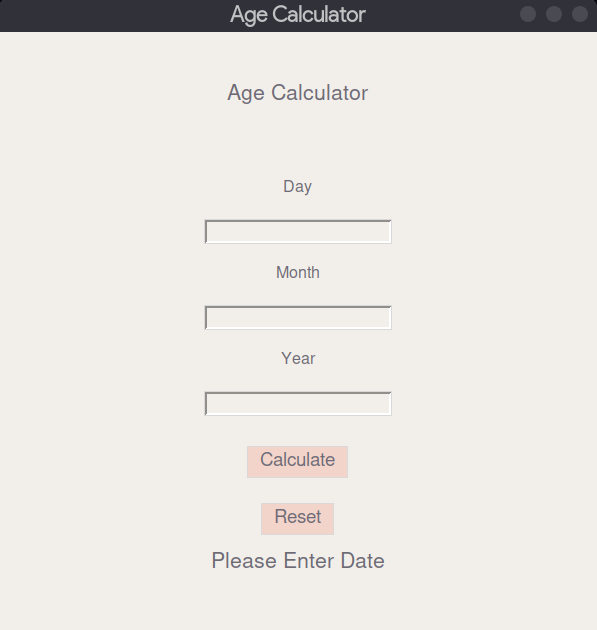
\includegraphics[width=.55\textwidth]{./Screenshot_on_2023-04-24_at_11-47-44.png}
    \caption{}
\end{figure}

\begin{figure}[H]
    \centering
    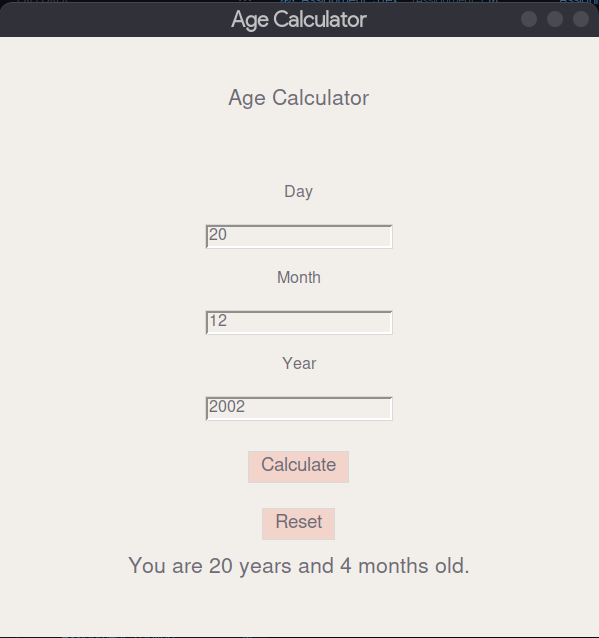
\includegraphics[width=.55\textwidth]{Screenshot_on_2023-04-24_at_11-48-02.png}
    \caption{}
\end{figure}

\begin{figure}[H]
    \centering
    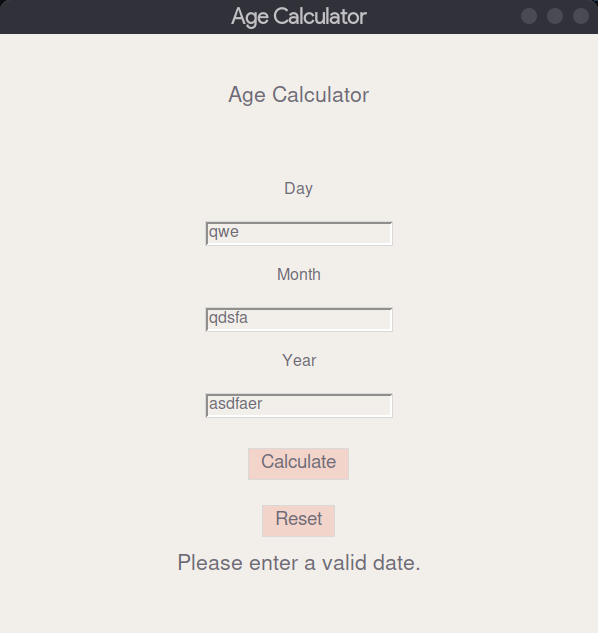
\includegraphics[width=.55\textwidth]{Screenshot_on_2023-04-24_at_11-48-21.png}
    \caption{}
\end{figure}

\section{Requirements}
\begin{enumerate}
    \item Python 3.7 or above
    \item tkinter module comes inbuilt with python
\end{enumerate}

\section{Code}

    \hypertarget{basic-tkinter-gui}{%
\subsection{Basic tkinter gui}\label{basic-tkinter-gui}}

    \begin{tcolorbox}[breakable, size=fbox, boxrule=1pt, pad at break*=1mm,colback=cellbackground, colframe=cellborder]
\prompt{In}{incolor}{24}{\boxspacing}
\begin{Verbatim}[commandchars=\\\{\}]
\PY{k+kn}{from} \PY{n+nn}{tkinter} \PY{k+kn}{import} \PY{o}{*}

\PY{c+c1}{\PYZsh{} size of the window is defined}
\PY{n}{root} \PY{o}{=} \PY{n}{Tk}\PY{p}{(}\PY{p}{)}
\PY{n}{root}\PY{o}{.}\PY{n}{geometry}\PY{p}{(}\PY{l+s+s2}{\PYZdq{}}\PY{l+s+s2}{400x400}\PY{l+s+s2}{\PYZdq{}}\PY{p}{)}

\PY{n}{frame\PYZus{}1} \PY{o}{=} \PY{n}{Frame}\PY{p}{(}\PY{n}{root}\PY{p}{)}
\PY{n}{frame\PYZus{}1}\PY{o}{.}\PY{n}{pack}\PY{p}{(}\PY{n}{side}\PY{o}{=}\PY{n}{TOP}\PY{p}{)}
\PY{n}{frame\PYZus{}2} \PY{o}{=} \PY{n}{Frame}\PY{p}{(}\PY{n}{root}\PY{p}{)}
\PY{n}{frame\PYZus{}2}\PY{o}{.}\PY{n}{pack}\PY{p}{(}\PY{n}{side}\PY{o}{=}\PY{n}{BOTTOM}\PY{p}{)}


\PY{n}{button\PYZus{}1} \PY{o}{=} \PY{n}{Button}\PY{p}{(}\PY{n}{frame\PYZus{}1}\PY{p}{,} \PY{n}{text}\PY{o}{=}\PY{l+s+s2}{\PYZdq{}}\PY{l+s+s2}{Button 1}\PY{l+s+s2}{\PYZdq{}}\PY{p}{,} \PY{n}{fg}\PY{o}{=}\PY{l+s+s2}{\PYZdq{}}\PY{l+s+s2}{red}\PY{l+s+s2}{\PYZdq{}}\PY{p}{)}
\PY{n}{button\PYZus{}2} \PY{o}{=} \PY{n}{Button}\PY{p}{(}\PY{n}{frame\PYZus{}1}\PY{p}{,} \PY{n}{text}\PY{o}{=}\PY{l+s+s2}{\PYZdq{}}\PY{l+s+s2}{Button 2}\PY{l+s+s2}{\PYZdq{}}\PY{p}{,} \PY{n}{fg}\PY{o}{=}\PY{l+s+s2}{\PYZdq{}}\PY{l+s+s2}{blue}\PY{l+s+s2}{\PYZdq{}}\PY{p}{)}

\PY{c+c1}{\PYZsh{} to add the button the respective screens}
\PY{n}{button\PYZus{}1}\PY{o}{.}\PY{n}{pack}\PY{p}{(}\PY{p}{)}
\PY{n}{button\PYZus{}2}\PY{o}{.}\PY{n}{pack}\PY{p}{(}\PY{p}{)}

\PY{n}{root}\PY{o}{.}\PY{n}{mainloop}\PY{p}{(}\PY{p}{)}
\end{Verbatim}
\end{tcolorbox}

    \hypertarget{assignment}{%
\subsection{Assignment}\label{assignment}}

    \begin{tcolorbox}[breakable, size=fbox, boxrule=1pt, pad at break*=1mm,colback=cellbackground, colframe=cellborder]
\prompt{In}{incolor}{25}{\boxspacing}
\begin{Verbatim}[commandchars=\\\{\}]
\PY{k+kn}{import} \PY{n+nn}{datetime}
\PY{k+kn}{import} \PY{n+nn}{tkinter} \PY{k}{as} \PY{n+nn}{tk}

\PY{c+c1}{\PYZsh{} Define the pastel color scheme}
\PY{n}{bg\PYZus{}color} \PY{o}{=} \PY{l+s+s2}{\PYZdq{}}\PY{l+s+s2}{\PYZsh{}F2EFEA}\PY{l+s+s2}{\PYZdq{}}
\PY{n}{fg\PYZus{}color} \PY{o}{=} \PY{l+s+s2}{\PYZdq{}}\PY{l+s+s2}{\PYZsh{}6D6A75}\PY{l+s+s2}{\PYZdq{}}
\PY{n}{button\PYZus{}color} \PY{o}{=} \PY{l+s+s2}{\PYZdq{}}\PY{l+s+s2}{\PYZsh{}F2D4CB}\PY{l+s+s2}{\PYZdq{}}
\PY{n}{button\PYZus{}hover\PYZus{}color} \PY{o}{=} \PY{l+s+s2}{\PYZdq{}}\PY{l+s+s2}{\PYZsh{}F2D4CB}\PY{l+s+s2}{\PYZdq{}}

\PY{k}{def} \PY{n+nf}{calculate\PYZus{}age}\PY{p}{(}\PY{p}{)}\PY{p}{:}
    \PY{c+c1}{\PYZsh{} get the current date}
    \PY{k}{try}\PY{p}{:} 
        \PY{n}{today} \PY{o}{=} \PY{n}{datetime}\PY{o}{.}\PY{n}{date}\PY{o}{.}\PY{n}{today}\PY{p}{(}\PY{p}{)}
        \PY{c+c1}{\PYZsh{} get the date of birth from the input fields}
        \PY{n}{day} \PY{o}{=} \PY{n+nb}{int}\PY{p}{(}\PY{n}{day\PYZus{}entry}\PY{o}{.}\PY{n}{get}\PY{p}{(}\PY{p}{)}\PY{p}{)}
        \PY{n}{month} \PY{o}{=} \PY{n+nb}{int}\PY{p}{(}\PY{n}{month\PYZus{}entry}\PY{o}{.}\PY{n}{get}\PY{p}{(}\PY{p}{)}\PY{p}{)}
        \PY{n}{year} \PY{o}{=} \PY{n+nb}{int}\PY{p}{(}\PY{n}{year\PYZus{}entry}\PY{o}{.}\PY{n}{get}\PY{p}{(}\PY{p}{)}\PY{p}{)}
        \PY{n+nb}{print}\PY{p}{(}\PY{n}{day}\PY{p}{,} \PY{n}{month}\PY{p}{,} \PY{n}{year}\PY{p}{)}
        \PY{n}{dob} \PY{o}{=} \PY{n}{datetime}\PY{o}{.}\PY{n}{date}\PY{p}{(}\PY{n}{year}\PY{p}{,} \PY{n}{month}\PY{p}{,} \PY{n}{day}\PY{p}{)}
        \PY{c+c1}{\PYZsh{} calculate the difference between the current date and date of birth}
        \PY{n}{age} \PY{o}{=} \PY{n}{today} \PY{o}{\PYZhy{}} \PY{n}{dob}
        \PY{c+c1}{\PYZsh{} calculate age in years and months}
        \PY{n}{years} \PY{o}{=} \PY{n+nb}{int}\PY{p}{(}\PY{n}{age}\PY{o}{.}\PY{n}{days} \PY{o}{/} \PY{l+m+mf}{365.25}\PY{p}{)}
        \PY{n}{months} \PY{o}{=} \PY{n+nb}{int}\PY{p}{(}\PY{p}{(}\PY{n}{age}\PY{o}{.}\PY{n}{days} \PY{o}{\PYZpc{}} \PY{l+m+mf}{365.25}\PY{p}{)} \PY{o}{/} \PY{l+m+mf}{30.44}\PY{p}{)}
        \PY{c+c1}{\PYZsh{} update the label with the age}
        \PY{n}{age\PYZus{}label}\PY{o}{.}\PY{n}{config}\PY{p}{(}\PY{n}{text}\PY{o}{=}\PY{l+s+s2}{\PYZdq{}}\PY{l+s+s2}{You are }\PY{l+s+si}{\PYZob{}\PYZcb{}}\PY{l+s+s2}{ years and }\PY{l+s+si}{\PYZob{}\PYZcb{}}\PY{l+s+s2}{ months old.}\PY{l+s+s2}{\PYZdq{}}\PY{o}{.}\PY{n}{format}\PY{p}{(}\PY{n}{years}\PY{p}{,} \PY{n}{months}\PY{p}{)}\PY{p}{)}
    \PY{k}{except}\PY{p}{:} 
        \PY{n}{age\PYZus{}label}\PY{o}{.}\PY{n}{config}\PY{p}{(}\PY{n}{text}\PY{o}{=}\PY{l+s+s2}{\PYZdq{}}\PY{l+s+s2}{Please enter a valid date.}\PY{l+s+s2}{\PYZdq{}}\PY{p}{)}

\PY{k}{def} \PY{n+nf}{reset\PYZus{}fields}\PY{p}{(}\PY{p}{)}\PY{p}{:}
    \PY{c+c1}{\PYZsh{} clear the input fields and age label}
    \PY{n}{day\PYZus{}entry}\PY{o}{.}\PY{n}{delete}\PY{p}{(}\PY{l+m+mi}{0}\PY{p}{,} \PY{n}{tk}\PY{o}{.}\PY{n}{END}\PY{p}{)}
    \PY{n}{month\PYZus{}entry}\PY{o}{.}\PY{n}{delete}\PY{p}{(}\PY{l+m+mi}{0}\PY{p}{,} \PY{n}{tk}\PY{o}{.}\PY{n}{END}\PY{p}{)}
    \PY{n}{year\PYZus{}entry}\PY{o}{.}\PY{n}{delete}\PY{p}{(}\PY{l+m+mi}{0}\PY{p}{,} \PY{n}{tk}\PY{o}{.}\PY{n}{END}\PY{p}{)}
    \PY{n}{age\PYZus{}label}\PY{o}{.}\PY{n}{config}\PY{p}{(}\PY{n}{text}\PY{o}{=}\PY{l+s+s2}{\PYZdq{}}\PY{l+s+s2}{\PYZdq{}}\PY{p}{)}

\PY{c+c1}{\PYZsh{} Create a new tkinter window}
\PY{n}{root} \PY{o}{=} \PY{n}{tk}\PY{o}{.}\PY{n}{Tk}\PY{p}{(}\PY{p}{)}
\PY{n}{root}\PY{o}{.}\PY{n}{title}\PY{p}{(}\PY{l+s+s2}{\PYZdq{}}\PY{l+s+s2}{Age Calculator}\PY{l+s+s2}{\PYZdq{}}\PY{p}{)}
\PY{n}{root}\PY{o}{.}\PY{n}{geometry}\PY{p}{(}\PY{l+s+s2}{\PYZdq{}}\PY{l+s+s2}{600x600}\PY{l+s+s2}{\PYZdq{}}\PY{p}{)}
\PY{n}{root}\PY{o}{.}\PY{n}{configure}\PY{p}{(}\PY{n}{bg}\PY{o}{=}\PY{n}{bg\PYZus{}color}\PY{p}{)}

\PY{n}{main\PYZus{}label} \PY{o}{=} \PY{n}{tk}\PY{o}{.}\PY{n}{Label}\PY{p}{(}\PY{n}{root}\PY{p}{,} \PY{n}{text}\PY{o}{=}\PY{l+s+s2}{\PYZdq{}}\PY{l+s+s2}{Age Calculator}\PY{l+s+s2}{\PYZdq{}}\PY{p}{,} \PY{n}{bg}\PY{o}{=}\PY{n}{bg\PYZus{}color}\PY{p}{,} \PY{n}{fg}\PY{o}{=}\PY{n}{fg\PYZus{}color}\PY{p}{,} \PY{n}{font}\PY{o}{=}\PY{p}{(}\PY{l+s+s2}{\PYZdq{}}\PY{l+s+s2}{Helvetica}\PY{l+s+s2}{\PYZdq{}}\PY{p}{,} \PY{l+m+mi}{16}\PY{p}{)}\PY{p}{)}
\PY{n}{main\PYZus{}label}\PY{o}{.}\PY{n}{pack}\PY{p}{(}\PY{n}{pady}\PY{o}{=}\PY{p}{(}\PY{l+m+mi}{50}\PY{p}{,} \PY{l+m+mi}{20}\PY{p}{)}\PY{p}{)}

\PY{c+c1}{\PYZsh{} Create the input fields for date of birth}
\PY{n}{day\PYZus{}label} \PY{o}{=} \PY{n}{tk}\PY{o}{.}\PY{n}{Label}\PY{p}{(}\PY{n}{root}\PY{p}{,} \PY{n}{text}\PY{o}{=}\PY{l+s+s2}{\PYZdq{}}\PY{l+s+s2}{Day}\PY{l+s+s2}{\PYZdq{}}\PY{p}{,} \PY{n}{bg}\PY{o}{=}\PY{n}{bg\PYZus{}color}\PY{p}{,} \PY{n}{fg}\PY{o}{=}\PY{n}{fg\PYZus{}color}\PY{p}{,} \PY{n}{font}\PY{o}{=}\PY{p}{(}\PY{l+s+s2}{\PYZdq{}}\PY{l+s+s2}{Helvetica}\PY{l+s+s2}{\PYZdq{}}\PY{p}{,} \PY{l+m+mi}{12}\PY{p}{)}\PY{p}{)}
\PY{n}{day\PYZus{}entry} \PY{o}{=} \PY{n}{tk}\PY{o}{.}\PY{n}{Entry}\PY{p}{(}\PY{n}{root}\PY{p}{,} \PY{n}{font}\PY{o}{=}\PY{p}{(}\PY{l+s+s2}{\PYZdq{}}\PY{l+s+s2}{Helvetica}\PY{l+s+s2}{\PYZdq{}}\PY{p}{,} \PY{l+m+mi}{12}\PY{p}{)}\PY{p}{,} \PY{n}{bg}\PY{o}{=}\PY{n}{bg\PYZus{}color}\PY{p}{,} \PY{n}{fg}\PY{o}{=}\PY{n}{fg\PYZus{}color}\PY{p}{,} \PY{n}{bd}\PY{o}{=}\PY{l+m+mi}{2}\PY{p}{)}
\PY{n}{month\PYZus{}label} \PY{o}{=} \PY{n}{tk}\PY{o}{.}\PY{n}{Label}\PY{p}{(}\PY{n}{root}\PY{p}{,} \PY{n}{text}\PY{o}{=}\PY{l+s+s2}{\PYZdq{}}\PY{l+s+s2}{Month}\PY{l+s+s2}{\PYZdq{}}\PY{p}{,} \PY{n}{bg}\PY{o}{=}\PY{n}{bg\PYZus{}color}\PY{p}{,} \PY{n}{fg}\PY{o}{=}\PY{n}{fg\PYZus{}color}\PY{p}{,} \PY{n}{font}\PY{o}{=}\PY{p}{(}\PY{l+s+s2}{\PYZdq{}}\PY{l+s+s2}{Helvetica}\PY{l+s+s2}{\PYZdq{}}\PY{p}{,} \PY{l+m+mi}{12}\PY{p}{)}\PY{p}{)}
\PY{n}{month\PYZus{}entry} \PY{o}{=} \PY{n}{tk}\PY{o}{.}\PY{n}{Entry}\PY{p}{(}\PY{n}{root}\PY{p}{,} \PY{n}{font}\PY{o}{=}\PY{p}{(}\PY{l+s+s2}{\PYZdq{}}\PY{l+s+s2}{Helvetica}\PY{l+s+s2}{\PYZdq{}}\PY{p}{,} \PY{l+m+mi}{12}\PY{p}{)}\PY{p}{,} \PY{n}{bg}\PY{o}{=}\PY{n}{bg\PYZus{}color}\PY{p}{,} \PY{n}{fg}\PY{o}{=}\PY{n}{fg\PYZus{}color}\PY{p}{,} \PY{n}{bd}\PY{o}{=}\PY{l+m+mi}{2}\PY{p}{)}
\PY{n}{year\PYZus{}label} \PY{o}{=} \PY{n}{tk}\PY{o}{.}\PY{n}{Label}\PY{p}{(}\PY{n}{root}\PY{p}{,} \PY{n}{text}\PY{o}{=}\PY{l+s+s2}{\PYZdq{}}\PY{l+s+s2}{Year}\PY{l+s+s2}{\PYZdq{}}\PY{p}{,} \PY{n}{bg}\PY{o}{=}\PY{n}{bg\PYZus{}color}\PY{p}{,} \PY{n}{fg}\PY{o}{=}\PY{n}{fg\PYZus{}color}\PY{p}{,} \PY{n}{font}\PY{o}{=}\PY{p}{(}\PY{l+s+s2}{\PYZdq{}}\PY{l+s+s2}{Helvetica}\PY{l+s+s2}{\PYZdq{}}\PY{p}{,} \PY{l+m+mi}{12}\PY{p}{)}\PY{p}{)}
\PY{n}{year\PYZus{}entry} \PY{o}{=} \PY{n}{tk}\PY{o}{.}\PY{n}{Entry}\PY{p}{(}\PY{n}{root}\PY{p}{,} \PY{n}{font}\PY{o}{=}\PY{p}{(}\PY{l+s+s2}{\PYZdq{}}\PY{l+s+s2}{Helvetica}\PY{l+s+s2}{\PYZdq{}}\PY{p}{,} \PY{l+m+mi}{12}\PY{p}{)}\PY{p}{,} \PY{n}{bg}\PY{o}{=}\PY{n}{bg\PYZus{}color}\PY{p}{,} \PY{n}{fg}\PY{o}{=}\PY{n}{fg\PYZus{}color}\PY{p}{,} \PY{n}{bd}\PY{o}{=}\PY{l+m+mi}{2}\PY{p}{)}

\PY{c+c1}{\PYZsh{} Create the button to calculate age}
\PY{n}{calc\PYZus{}button} \PY{o}{=} \PY{n}{tk}\PY{o}{.}\PY{n}{Button}\PY{p}{(}\PY{n}{root}\PY{p}{,} \PY{n}{text}\PY{o}{=}\PY{l+s+s2}{\PYZdq{}}\PY{l+s+s2}{Calculate}\PY{l+s+s2}{\PYZdq{}}\PY{p}{,} \PY{n}{bg}\PY{o}{=}\PY{n}{button\PYZus{}color}\PY{p}{,} \PY{n}{fg}\PY{o}{=}\PY{n}{fg\PYZus{}color}\PY{p}{,} \PY{n}{font}\PY{o}{=}\PY{p}{(}\PY{l+s+s2}{\PYZdq{}}\PY{l+s+s2}{Helvetica}\PY{l+s+s2}{\PYZdq{}}\PY{p}{,} \PY{l+m+mi}{14}\PY{p}{)}\PY{p}{,} \PY{n}{bd}\PY{o}{=}\PY{l+m+mi}{0}\PY{p}{,}
                        \PY{n}{activebackground}\PY{o}{=}\PY{n}{button\PYZus{}hover\PYZus{}color}\PY{p}{,} \PY{n}{activeforeground}\PY{o}{=}\PY{n}{fg\PYZus{}color}\PY{p}{,} \PY{n}{command}\PY{o}{=}\PY{n}{calculate\PYZus{}age}\PY{p}{)}


\PY{c+c1}{\PYZsh{} Create the button to reset the fields}
\PY{n}{reset\PYZus{}button} \PY{o}{=} \PY{n}{tk}\PY{o}{.}\PY{n}{Button}\PY{p}{(}\PY{n}{root}\PY{p}{,} \PY{n}{text}\PY{o}{=}\PY{l+s+s2}{\PYZdq{}}\PY{l+s+s2}{Reset}\PY{l+s+s2}{\PYZdq{}}\PY{p}{,} \PY{n}{bg}\PY{o}{=}\PY{n}{button\PYZus{}color}\PY{p}{,} \PY{n}{fg}\PY{o}{=}\PY{n}{fg\PYZus{}color}\PY{p}{,} \PY{n}{font}\PY{o}{=}\PY{p}{(}\PY{l+s+s2}{\PYZdq{}}\PY{l+s+s2}{Helvetica}\PY{l+s+s2}{\PYZdq{}}\PY{p}{,} \PY{l+m+mi}{14}\PY{p}{)}\PY{p}{,} \PY{n}{bd}\PY{o}{=}\PY{l+m+mi}{0}\PY{p}{,}
                         \PY{n}{activebackground}\PY{o}{=}\PY{n}{button\PYZus{}hover\PYZus{}color}\PY{p}{,} \PY{n}{activeforeground}\PY{o}{=}\PY{n}{fg\PYZus{}color}\PY{p}{,} \PY{n}{command}\PY{o}{=}\PY{n}{reset\PYZus{}fields}\PY{p}{)}


\PY{c+c1}{\PYZsh{} Create the label to display the age}
\PY{n}{age\PYZus{}label} \PY{o}{=} \PY{n}{tk}\PY{o}{.}\PY{n}{Label}\PY{p}{(}\PY{n}{root}\PY{p}{,} \PY{n}{text}\PY{o}{=}\PY{l+s+s2}{\PYZdq{}}\PY{l+s+s2}{Please Enter Date}\PY{l+s+s2}{\PYZdq{}}\PY{p}{,} \PY{n}{bg}\PY{o}{=}\PY{n}{bg\PYZus{}color}\PY{p}{,} \PY{n}{fg}\PY{o}{=}\PY{n}{fg\PYZus{}color}\PY{p}{,} \PY{n}{font}\PY{o}{=}\PY{p}{(}\PY{l+s+s2}{\PYZdq{}}\PY{l+s+s2}{Helvetica}\PY{l+s+s2}{\PYZdq{}}\PY{p}{,} \PY{l+m+mi}{16}\PY{p}{)}\PY{p}{)}

\PY{c+c1}{\PYZsh{} Add the widgets to the window}
\PY{n}{day\PYZus{}label}\PY{o}{.}\PY{n}{pack}\PY{p}{(}\PY{n}{pady}\PY{o}{=}\PY{p}{(}\PY{l+m+mi}{50}\PY{p}{,} \PY{l+m+mi}{10}\PY{p}{)}\PY{p}{)}
\PY{n}{day\PYZus{}entry}\PY{o}{.}\PY{n}{pack}\PY{p}{(}\PY{n}{pady}\PY{o}{=}\PY{l+m+mi}{10}\PY{p}{)}
\PY{n}{month\PYZus{}label}\PY{o}{.}\PY{n}{pack}\PY{p}{(}\PY{n}{pady}\PY{o}{=}\PY{l+m+mi}{10}\PY{p}{)}
\PY{n}{month\PYZus{}entry}\PY{o}{.}\PY{n}{pack}\PY{p}{(}\PY{n}{pady}\PY{o}{=}\PY{l+m+mi}{10}\PY{p}{)}
\PY{n}{year\PYZus{}label}\PY{o}{.}\PY{n}{pack}\PY{p}{(}\PY{n}{pady}\PY{o}{=}\PY{l+m+mi}{10}\PY{p}{)}
\PY{n}{year\PYZus{}entry}\PY{o}{.}\PY{n}{pack}\PY{p}{(}\PY{n}{pady}\PY{o}{=}\PY{l+m+mi}{10}\PY{p}{)}
\PY{n}{calc\PYZus{}button}\PY{o}{.}\PY{n}{pack}\PY{p}{(}\PY{n}{pady}\PY{o}{=}\PY{l+m+mi}{20}\PY{p}{)}
\PY{n}{reset\PYZus{}button}\PY{o}{.}\PY{n}{pack}\PY{p}{(}\PY{n}{pady}\PY{o}{=}\PY{l+m+mi}{5}\PY{p}{)}
\PY{n}{age\PYZus{}label}\PY{o}{.}\PY{n}{pack}\PY{p}{(}\PY{n}{pady}\PY{o}{=}\PY{l+m+mi}{10}\PY{p}{)}

\PY{c+c1}{\PYZsh{} Run the main tkinter event loop}
\PY{n}{root}\PY{o}{.}\PY{n}{mainloop}\PY{p}{(}\PY{p}{)}
\end{Verbatim}
\end{tcolorbox}

    \begin{Verbatim}[commandchars=\\\{\}]
20 12 2002
    \end{Verbatim}

    \begin{tcolorbox}[breakable, size=fbox, boxrule=1pt, pad at break*=1mm,colback=cellbackground, colframe=cellborder]
\prompt{In}{incolor}{ }{\boxspacing}
\begin{Verbatim}[commandchars=\\\{\}]

\end{Verbatim}
\end{tcolorbox}

    
\section{Conclusion}
Studied Python GUI using Tkinter with various widgets.

\clearpage

\section{FAQ}
\begin{enumerate}
\item \textbf{What is python Tkinter?}\\

Tkinter is a Python binding to the Tk GUI toolkit. It is the standard Python interface to the Tk GUI toolkit, and is Python's de facto standard GUI.
It is a thin object-oriented layer on top of Tcl/Tk. Tkinter is not the only GuiProgramming toolkit for Python. It is however the most commonly used one, and almost the only one that is portable between Unix, Mac and Windows. It was originally written for Python 1.4, and is now the standard way to create a GUI with Python. \\

There are also other GUI toolkits like wxPython, PyQt, Kivy, etc. \\

\item \textbf{What is Python Tkinter pack() and mainloop() method?}\\

pack() method: This geometry manager organizes widgets in blocks before placing them in the parent widget.\\

mainloop() method: There is a method known by the name mainloop() is used when your application is ready to run. mainloop() is an infinite loop used to run the application, wait for an event to occur and process the event as long as the window is not closed.\\

\begin{lstlisting}[language=python]
# Python program to create a simple GUI and show an example of pack() method and mainloop() method

# Importing Tkinter module
from tkinter import *

root = Tk()

# Creating a Label Widget
myLabel1 = Label(root, text="Hello World!")

# Showing it onto the screen
myLabel1.pack()

# Creating a Label Widget
myLabel2 = Label(root, text="My name is John Elder")

# Showing it onto the screen
myLabel2.pack()

root.mainloop() // runs in a infinite loop

\end{lstlisting}

\end{enumerate}


\end{document}